\chapter{Implementation}
\label{chapter:implementation}
% \epigraph{The best presents don't come in boxes.}{Bill Watterson}
% \epigraph{Typing is no substitute for thinking.}{Dartmouth Basic manual, 1964}

This chapter is divided into two parts.
The first half of this chapter will describe the methods used to execute TASTy in a Truffle interpreter.
Section \ref{impl:section:execution} will cover how to tranform the semantics of TASTy to Truffle AST nodes.
In particular, the first section focuses how to translate the organization of data and code in \scalainline{DefDef}, \scalainline{ClassDef}, and \scalainline{Term} trees into an Truffle implementation which is executable.
The first half of this chapter will omit the discussion of translating \scalainline{TypeDef}, \scalainline{TypeTree} and \scalainline{Type} constructs in general. 
The second half of this chapter covers the techniques we will use to eliminate autoboxing Truffle itself is unable to eliminate. 

\section{Execution}
\label{impl:section:execution}

Scala programs in \acrshort{tasty} format are unsuitable for execution in a Truffle interpreter. 
Programs in must be parsed and transformed into an executable representation in \textsc{TastyTruffle}. 
As TASTy represents a Scala program close to its equivalent source representation, canonicalization compiler passes (see appendix \ref{appendix:dotty-phases}) that would otherwise normalize the IR are not present. 
Instead, we implement TastyTruffle IR to represent a canonicalized executable intermediate representation which can be specialized on demand. 

In the following sections, we will describe the individual types of TASTy nodes and why some are directly unsuitable for execution and how to simplify their semantics for execution.
We will begin with a explanation of how data is encoded and defined in TASTy.

\subsection{Converting the \texttt{DefDef} tree into a Truffle Root Node}
\label{impl:subsection:defdef}

In this section, we describe the conversion of \scalainline{DefDef} trees to \textit{root nodes}.
\scalainline{DefDef} trees are the primary structure which organizes code (terms) in TASTY.
Root nodes represent the root of an executable Truffle AST, the primary structure which organizes code in Truffle.
In our case, root nodes are the Truffle analog of a \scalainline{DefDef}.
Each root node has a corresponding \textit{call target}, which is used for invocation of the root node.
A root node is automatically instrumented\cite{profiling:atom} to profile its number of invocations. 

\begin{figure}[!htb]
	\begin{minted}{scala}
	abstract class RootNode(desc: FrameDescriptor) {
		def execute(frame: VirtualFrame): Object
		def getCallTarget: CallTarget
	}
	\end{minted}
	\caption{Pseudocode of a root node.}
	\label{example:root-node}
\end{figure}

Figure \ref{example:root-node} gives a simplified implementation of a root node.
Each root node in Truffle has a \textit{frame descriptor} and execution semantics.
A guest language must subclass and implement its own root node in order to enable function invocation semantics.

A frame descriptor describes guest language variables which are in scope during execution.
The abstract \javainline{execute} method describes the invocation behaviour of a root node.
When a root node is executed, it always supplied with a \textit{frame}.
A frame contains the arguments supplied during invocation and storage slots for local variable definitions in the body of the method.
By default, all frames in execution are \textit{virtual}.
Virtual frames are an Truffle abstraction which provides guest languages an opportunity to exploit escape analysis.
Escape analysis\cite{escape-analysis} reasons about the dynamic scope of object allocations. 
Truffle and Graal both exploit the observations of \textit{Partial Escape Analysis}\cite{java:partial-escape-analysis}, a path-sensitive variant of escape analysis, to enable the following optimizations for guest languages:

\begin{description}
	\item[Region Allocation\cite{java:escape-analysis}\cite{tofte:region-memory}] The substitution of heap allocations with stack allocations to eliminate unnecessary garbage collection.
	\item[Scalar Replacement\cite{java:escape-analysis-optimizations}] The complete elimination of an object allocation, where the fields of the replaced object are substituted by local variables.
\end{description}

The virtual frame abstraction allow guest languages to read and write normally without having to optimize their object allocations.
Escape analysis occurs automatically during partial evaluation with no guest language intervention necessary. 

\begin{figure}[!htb]
	\begin{minted}{scala}
	class DefDef(_: String, params: List[ParamClause], _: TypeTree, rhs: Option[Term]) extends Definition	
	\end{minted}
	\caption{Defintion of a \texttt{DefDef} tree with names of less important members replaced with \texttt{\_}}
	\label{recall:defdef}
\end{figure}

A further simplified definition of a \scalainline{DefDef} tree is provided in figure \ref{recall:defdef}.
In this section, we focus on two members of a \scalainline{DefDef} trees.
The parameters of a \scalainline{DefDef} tree are given by the \scalainline{params} field.
In practice, the type of a \scalainline{ParamClause} is an alias for the union type \scalainline{TypeParams {|} TermParams}, so we omit the \scalainline{ParamClause} definition.
A \scalainline{DefDef} tree will have a parameter section for type parameters when they are polymorphic and will always have term parameters section.
\scalainline{DefDef} trees may optionally have a body defined in the \scalainline{rhs} field.
When trees do not have a body defined, they are abstract method definitions and do not have corresponding root node in Truffle.
We will only consider non-abstract method definitions which have a body (a term) defined to be executable.
We will cover the parsing of terms into nodes for execution in detail after section \ref{impl:subsection:classdef}

\begin{figure}[!htb]
	\begin{minted}{scala}
	object FrameSlotKind extends Enumeration {
		type FrameSlotKind = Value
		val Object, Long, Int, Double, Float, Boolean, Byte = Value
	}	
		
	def getFrameSlotKind(tpe: Type): FrameSlotKind = 
		if (tpe.isPrimitive) 
			getPrimitiveSlotKind(tpe) // Int => FrameSlotKind.Int, ..., Double => FrameSlotKind.Double
		else  
			FrameSlotKind.Object
	\end{minted}
	\caption{Simplified implementation of \scalainline{FrameSlotKind}}
	\label{impl:frameslot-kind}
\end{figure}

Each value definition in the parameters of a \scalainline{DefDef} will have a corresponding frame slot in its parent frame descriptor. 
A frame slot references a unique frame value in the context of a root node.
Truffle permits each frame slot in a frame descriptor be described by a \textit{frame slot kind}.
In Truffle, there is a corresponding frame slot kind for reference types and each \acrshort{jvm} primitive type. 
Pseudocode of a frame slot kind and a method to convert a type into a slot kind is given in \ref{impl:frameslot-kind}.

Truffle profiles frame accesses in order to minimize the amount of autoboxing which occurs when reading from frame slot with an \javainline{Object} kind. 
To eliminate unnecessary specialization of frame accesses where types are monomorphic and statically refer to a primitive type, a parameter is assigned the matching primitive frame slot kind in the frame descriptor. 
In cases where the type is not a primitive type or a polymorphic applied type, e.g. \scalainline{List[T]} but not \scalainline{T}, we assign its frame slot the \scalainline{Object} kind.
Otherwise, the type is a polymorphic parameter which \textit{could} resolve to a primitive type and the frame slot kind cannot be resolved statically.
We will defer discussion on how to handle parameters of such polymorphic types that cannot be resolved statically until section \ref{implementation:specialization}.


\begin{figure}[!htb]
	\begin{minted}{scala}
	case class Parameter(slot: FrameSlot, kind: FrameSlotKind)
		
	class DefDefNode(desc: FrameDescriptor, params: Array[Parameter], body: TermNode) extends RootNode(desc) {
		override def execute(frame: VirtualFrame): Object = {
			copyArgumentsToFrame(frame)
			body.execute()
		}	
			
		def copyArgumentsToFrame(frame: VirtualFrame): Unit = 
			for ((param, arg) <- params zip frame.getArguments) 
				param.kind match {
					case FrameSlotKind.Int =>
						frame.setInt(param.slot, arg.asInstanceOf[Int])
					...
					case FrameSlotKind.Double =>
						frame.setDouble(param.slot, arg.asInstanceOf[Double])	
					case _ =>
						frame.setObject(param.slot, arg)
				}
	}
	\end{minted}
	\caption{Pseudocode for \scalainline{DefDefNode} and \scalainline{Parameter}}
	\label{impl:defdefnode}
\end{figure}

Figure \ref{impl:defdefnode} provides the implementation of the \scalainline{DefDefNode} and its parameters, the root node equivalent of a \scalainline{DefDef}.
The execution of a \scalainline{DefDefNode} is divided into two stages, argument preparation and execution.
First, the arguments of the frame constructed during invocation (see \ref{impl:subsection:apply}), are copied into their respective parameter frame slots.
Frames contains separate regions for values of each frame slot kind.
Based on the frame slot kind prescribed to a parameter, we copy each argument into the appropriate frame slot region.
Storing parameters in this manner eliminates any unnecessary unboxing which would otherwise occur during a frame access.
After arguments are copied into the frame, their values become available for access during the execution of the body.
The body of a \scalainline{DefDefNode} is then executed and its computed value returned .

\begin{figure}[!htb]
	\begin{minted}{scala}
	def parse(ddef: DefDef): DefDefNode = {
		val desc = new FrameDescriptor
		val parameters = 
			self :: ddef.params.map {
				case vdef: ValDef => createParameter(valDef, desc)
			}
			
		val body = parse(definition.rhs)
		new DefDefNode(desc, parameters, body)
		}
		
	def createParam(vdef: ValDef, desc: FrameDescriptor): Parameter = {
		val kind = getFrameSlotKind(vdef.tpt.tpe)
		val slot = desc.addSlot(kind)
		Parameter(slot, kind)
	}
	\end{minted}
	\caption{Pseudocode for parsing \scalainline{DefDef} into \scalainline{DefDefNode}}
	\label{impl:parse-defdef}
\end{figure}

Figure \ref{impl:parse-defdef} provides a summary on parsing a \scalainline{DefDef} tree into its Truffle equivalent \scalainline{DefDefNode}.
Frame slot and a frame slot kinds provide an abstraction for parameters and arguments to be resolved before the execution of the main body in a \scalainline{DefDefNode}.
In addition to the parameters which are explictly present in TASTY, the root node will have additional parameter which represents the receiver of the method.
The receiver is an object instance whose class definition owns the method being invoked.
In Scala, every method invocation has a receiver.
In TASTy, this translates to every \scalainline{DefDef} is owned by a \scalainline{ClassDef}.
In the next section, we detail how to organize call targets in Truffle by using \scalainline{ClassDef} trees.

\section{Deriving Shapes from \texttt{ClassDef} trees}

\begin{figure}[!htb]
	\centering
	\begin{subfigure}[b]{0.48\textwidth}
	\begin{minted}{scala}
	class ClassDef(
		name:        String,
		constructor: DefDef, 
		parents:     List[Tree], 
		_:           Option[ValDef], 
		body:        List[Statement]
	) extends Definition
		\end{minted}
	\caption{Pseudocdoe of a \scalainline{ClassDef}.}
	\label{recall:classdef}
	\end{subfigure}
	\hfill
	\begin{subfigure}[b]{0.48\textwidth}
	\begin{minted}{scala}
	class ClassShape(
		symbol:  Symbol,
		parents: Array[Symbol],
		fields:  Array[Field]
		methods: Map[MethodSignature, CallTarget]
		vtable:  Map[MethodSignature, Symbol]
	)
	\end{minted}
	\caption{Pseudocode of a shape for a \scalainline{ClassDef}.}
	\label{impl:classshape}
	\end{subfigure}
\end{figure}

\scalainline{ClassDef} tree define the layout of an object in TASTy.
The layout of a object dictate the values which an object instance stores as well the methods which can be invoked on an object instance.
The data layout of an object in a Truffle interpreter is described by a \textit{shape}\cite{self:prototypes}\cite{truffle:object-model}.
Shapes are a language-agnostic model for defining the properties of a object instance in Truffle.
A property in a shape describes one member of an object instance; it has an identifier and a value.
A Truffle object instance consists of \textit{object storage}, which contains instance-specific data, and its shape.
Shapes map property identifiers to object storage locations; guest languages interface with object storage indirectly through properties.
In this thesis we use a \textit{static shape}, an immutable variant of a shape.
Normally, shapes are mutable and their list of properties may change throughout the lifetime of a program\cite{truffleruby:object-model}.
However, programs which dynamically change the layout of their objects\cite{java:reflection} are out of the scope of this thesis.

\begin{figure}[!htb]
	\begin{minted}{scala}
	def parse(cdef: ClassDef): ClassShape = {
		val parents = cdef.parents.map(_.symbol)
		
		val fields = cdef.body map {
			case vdef: ValDef => generateField(vdef)	
		}
	
		val initializer = 
	
		val methods = def.body map {
			case ddef: DefDef => ddef.symbol.signature -> parse(ddef)
		}
		
		val vtable = cdef.symbol.methodMembers map {
			symbol => symbol.signature -> symbol
		}
	
		new ClassShape(cdef.symbol, parents, fields, methods, vtable)
	}

	def generateField(vdef: ValDef): Field = vdef match {
		case ValDef(_: String, tpt: TypeTree, rhs: Option[Term]) => new Field(vdef.symbol, )
	}
	\end{minted}
	\caption{Pseudocodeto convert a \scalainline{ClassDef} into a \scalainline{ClassShape}.}
	\label{impl:parse-classdef}
\end{figure}


Recall the definition of a \scalainline{ClassDef} in figure \ref{recall:classdef}.
Each \scalainline{ClassDef} tree can be parsed into a corresponding \scalainline{ClassShape}, given in Figure \ref{impl:classshape}.
The \scalainline{name} parameter of \scalainline{ClassDef} is insufficient to be used as an identifier for a \scalainline{ClassShape}.
Names do not disambiguate between classes of the same name declared in different packages.
Instead, we used the symbol of the \scalainline{ClassDef} tree as the identifier for the \scalainline{ClassShape}.
A \scalainline{ValDef} tree in the body of a \


\begin{figure}[!htb]
	\begin{minted}{scala}
	class Field(symbol: Symbol, tpe: Type) extends StaticProperty {
		override def getId: String = symbol.name
			
		def get(instance: Object): Any = 
			if (tpe == Int) getInt(instance)
			else if ...
			else if (tpe == Double) getDouble(instance)
			else getObject(instance)
	
			
		def set(instance: Object, value: Any): Unit = 
			if (tpe == Int) setInt(instance, value.asInstanceOf[Int])
			else if ...
			else if (tpe == Double) setDouble(instance, value.asInstanceOf[Double])
			else setObject(instance, value)	
	} 
	\end{minted}
	\caption{Pseudocode of the field property.}
	\label{impl:field}
\end{figure}

For the remainder of this thesis, we will use a \scalainline{ClassInstance} to refer to an object instance with properties described by a \scalainline{ClassShape}.
A \scalainline{ClassShape} has an collection of fields, which are implementations of a static shape property.
Figure \ref{impl:field} gives our implementation of a field.
Fields define operations to read and write from the object storage on a \scalainline{ClassInstance}.
Like frames with frame slot kinds, object instances in Truffle have separate regions for storing values of each primitive type and one for reference types.
Following the same rules with types and frame slot kinds described in section \ref{impl:subsection:defdef}, the data access of a field depends on the type of the \scalainline{ValDef} tree from which the field originates.
The remaining members of a \scalainline{ClassShape} do not describe data which has to be stored in the object storage of a \scalainline{ClassInstance}.

\begin{figure}[!htb]
	\begin{minted}{scala}
	case class MethodSignature(symbol: Symbol, params: Int, types: Array[Type])
	\end{minted}
	\caption{Pseudocode of a method signature.}
	\label{impl:method-signature}
\end{figure}

After the constructor and the \scalainline{DefDef} statements of a \scalainline{ClassDef} are converted into root nodes, they are stored in the \scalainline{ClassShape} mapped by a method signature.
The pseudocode for a method signature is given in figure \ref{impl:method-signature}.
Method signatures disambiguate method invocations in the presence of \textit{ad hoc polymorphism}\cite{strachey:fundamental-concepts}, where methods share the same name but have different arguments.
When combined with parametric polymorphism, method signatures must also be able to disamibguate between methods sharing the same name but having different type parameters.
However, method signatures do not have to disambiguate between different type parameters by name, only the number of type parameters that a method has.
Because type erasure erases polymorphic type parameters from methods, methods which share the same number of parameters as well as the same arguments will conflict and therefore are invalid.
As previously mentioned, methods are shared between all \scalainline{ClassInstance} objects with the same shape, call targets are stored on the shape itself.

Often, a shape will not contain the call target referenced by a signature because the dispatch is dynamic.
A \scalainline{ClassShape} contains a \textit{virtual method table}, which maps a method signature to the symbol of a shape which contains the call target matching the signature.
If a method signature does not have a call target in the current shape, the shape which holds the target is indirectly resolved using the virtual method table during execution.

\subsection{Creating Instances with the \texttt{New} Tree}

\subsection{Disambiguating \texttt{Apply} trees}
\label{impl:subsection:apply}
The \scalainline{Apply} tree is a context-sensitive tree which represents multiple types of operations:

\begin{description}
	\item[Method invocation] description
	\item[Array access]
	\item[Arithmetic and Logical Operators]
\end{description}

\subsubsection*{Method Invocation}

\begin{figure}[!htb]
	\begin{minted}{scala}
	class ApplyNode(sig: MethodSignature, receiver: TermNode, args: Array[TermNode]) extends TermNode {
		final val INLINE_CACHE_SIZE: Int = 5;
		
		@Specialization(guards = "inst.type == tpe", limit = "INLINE_CACHE_SIZE")
		def cached(
			frame: VirtualFrame,
			inst: ClassInstance,
			@Cached("inst.type") tpe: Type,
			@Cached("create(resolveCall(instance, sig)") callNode: DirectCallNode
		): Object = callNode.call(evalArgs(frame, inst));
		
		@Specialization(replaces = "cached")
		def virtual(
			frame: VirtualFrame,
			inst: ClassInstance,
			@Cached callNode: IndirectCallNode
		): Object = {
			val callTarget = resolveCall(instance, sig);
			callNode.call(callTarget, evalArgs(frame, inst))
		}
	}
	\end{minted}
	\caption{Simplified implementation of the call node with a polymorphic inline cache used in TastyTruffle.}
	\label{implementation:poly-cache-call-node}
\end{figure}

Method invocations exists in multiple forms because tree canocalization happens immediately after the TASTy picking phase in the compilation pipeline.
The result is that TASTy trees retain some syntactic elements from their Scala sources. 
For example, Truffle provides two abstractions for call nodes, the \textit{direct call node} is used when the call target can be statically resolved. 
In TASTy, this includes the set of methods with private or final modifiers\cite{java:lang-spec} and class constructors. 
Otherwise, the \textit{indirect call node} is used for calls which have dynamically resolved call targets. 
\textsc{TastyTruffle} uses a singular call node implementation for both monomorphic and polymorhic calls. 
we utilize a polymorphic inline cache\cite{self:polymorphic-inline-caches} to eliminate the overhead of resolving polymorphic calls for \acrshort{jit} compilation. 
Figure \ref{implementation:poly-cache-call-node} shows a simplified Truffle call node in \textsc{TastyTruffle} which implements a polymorphic inline cache.

\begin{figure}[!htb]
	\centering
	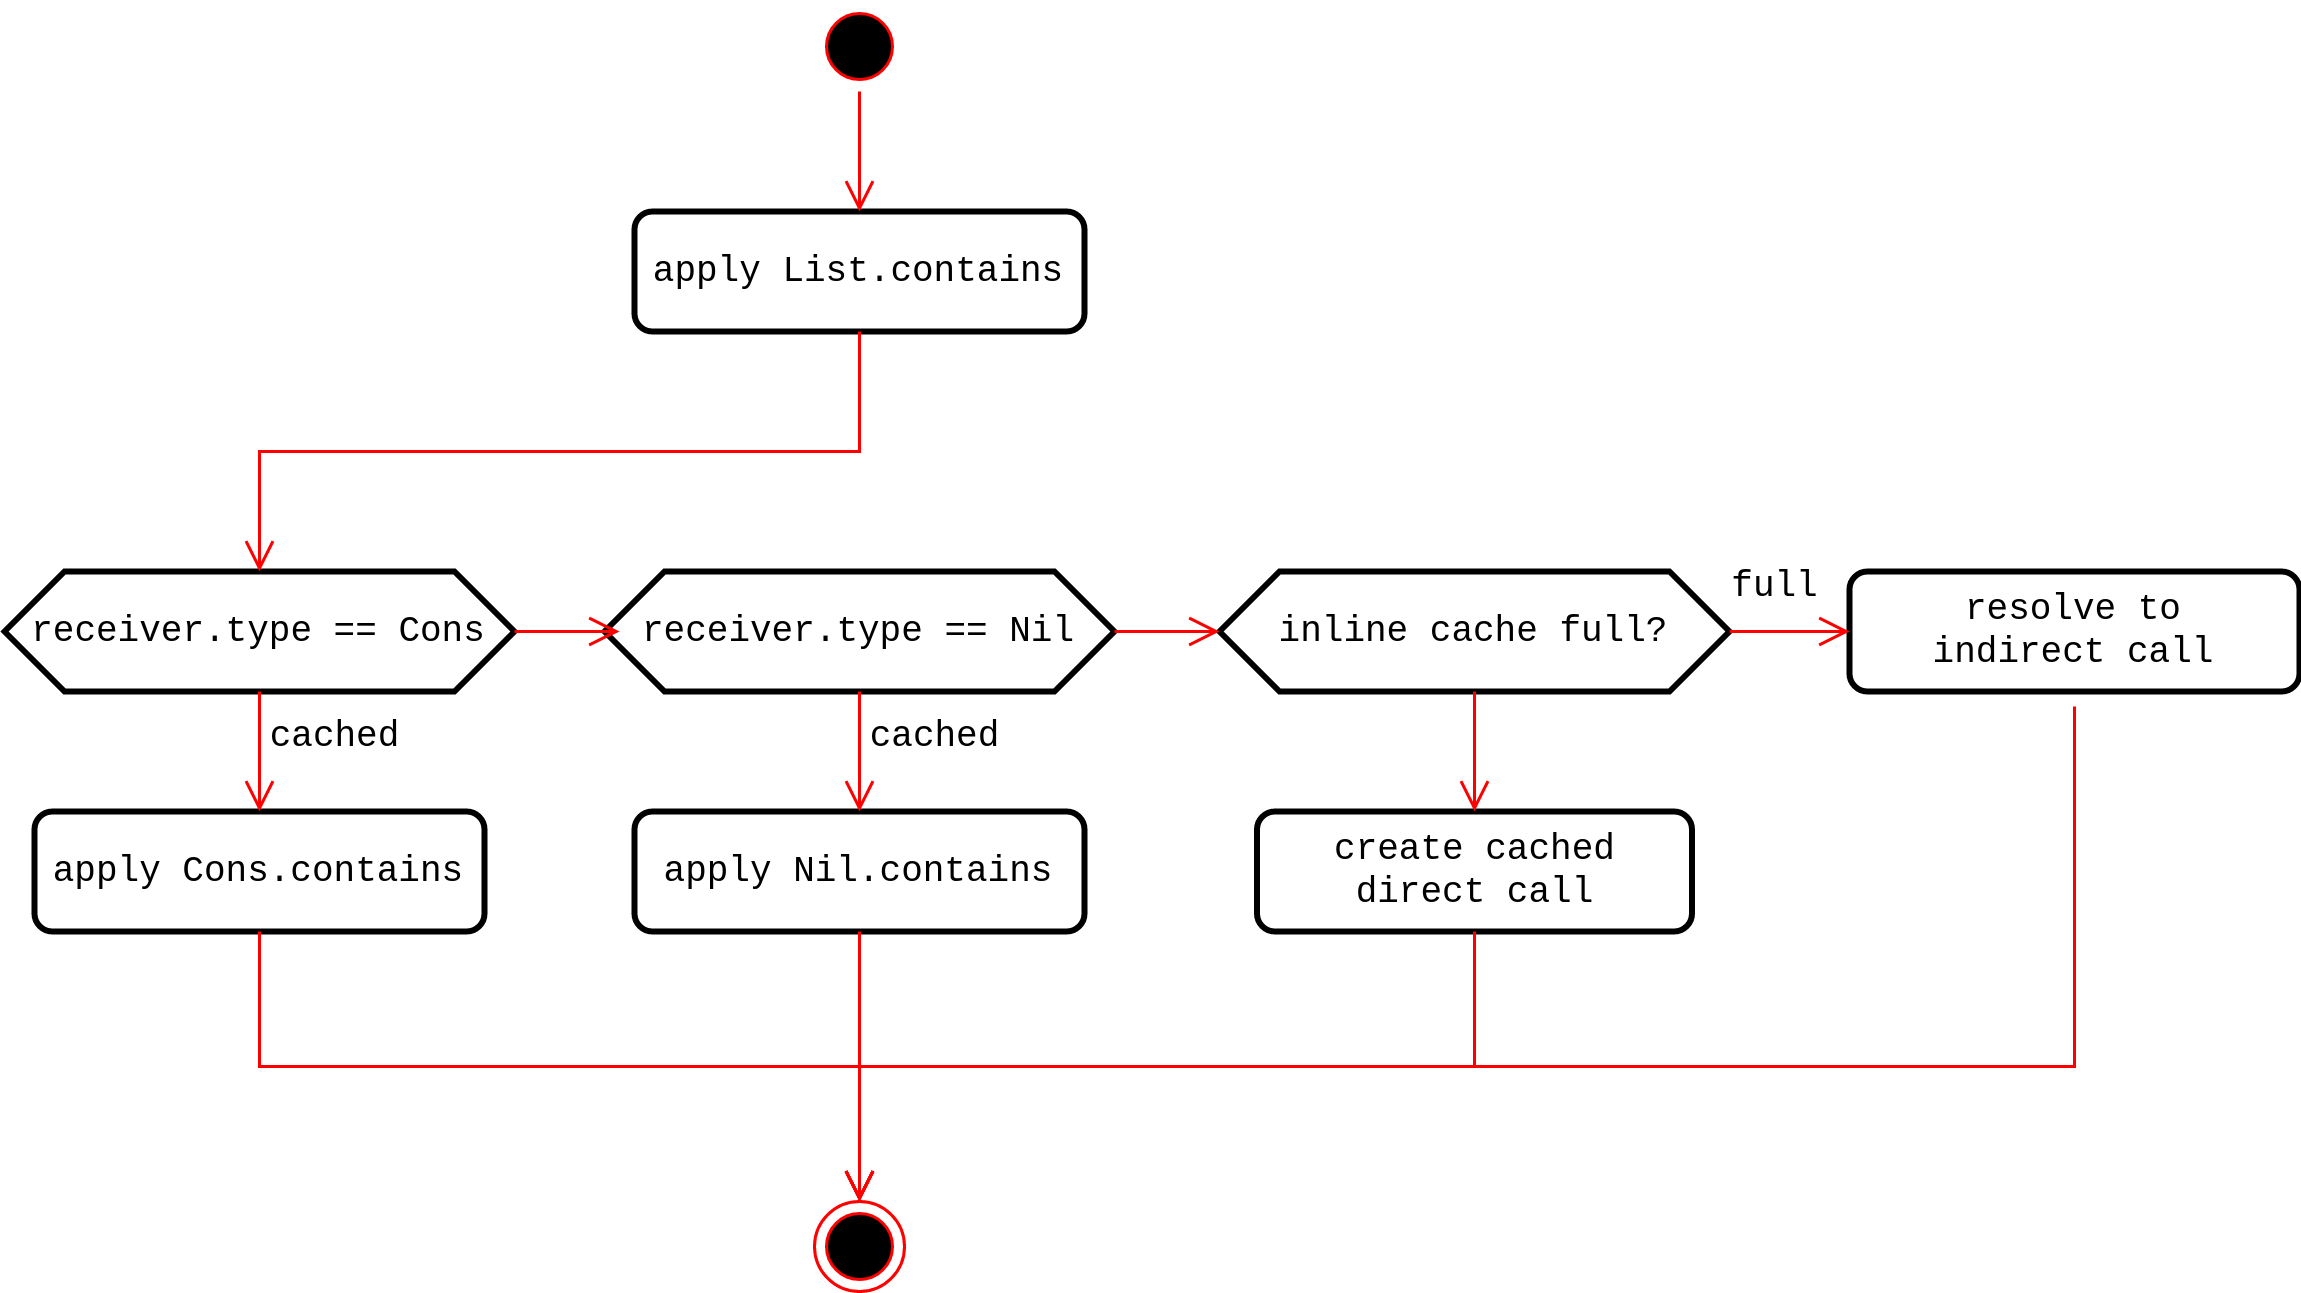
\includegraphics[width=0.6\textwidth]{figures/tastytruffle-pic-example.png}
	\caption{A possible polymorphic inline cache for a \scalainline{List.contains} callsite.}
	\label{example:poly-cache-call-node}
\end{figure}

The Truffle \acrshort{dsl} emits a cache which is searched linearly based on the type of receiver. 
When the type of receiver has not been seen in the inline cache, an additional cache entry is generated and appended to the cache for the next call. 
The size of an polymorphic inline cache must be kept reasonable ???. 
The generated inline cache can be used to inline code and JIT optimized based on the type of the receiver seen at a call site. 

When the polymorphic inline cache is applied to a monomorphic call site, it simplifies to a single element inline cache\cite{smalltalk:inline-caches}. 
Because the type of the receiver at the call site remains stable, the cache look up of the call target based on the type always succeeds and the call site never fallbacks to using an indirect call node.

\subsubsection{Unary and Binary Expressions}

Unary and Binary operations in Scala are syntactic sugar for function invocation. 
For example, the following addition \scalainline{1 + 2} is desugared to \scalainline{1.+(2)}. 
That is, the binary operator \scalainline{+} is represented as the invocation of the instance function \scalainline{Int.+} on the receiver with value \scalainline{1} and type \scalainline{Int} with a single argument \scalainline{2}.
Normally in the Scala compilation pipeline, methods which operate on primtive types and have an underlying implementation on the JVM\cite{java:vm-spec}, e.g. in a bytecode instruction, are replaced by those instructions in compiled program bytecode. 
Similarly, TastyTruffle avoids implementing methods of primitive types with actual call semantcs as primitive operations are frequently used and simple to optimize as instrinsic implementations exist on many Java virtual machines.\cite{???}

\subsection{The \texttt{Block} tree}

\subsection{Generating Frame Slots from \texttt{ValDef} trees} 

The \scalainline{ValDef} tree is a multi-purpose node which represents value definitions in many contexts.
This section will only cover the \scalainline{ValDef} tree in the context of local variables.
Sections \ref{impl:subsection:defdef} and \ref{impl:subsection:classdef} will cover the remaining contexts where \scalainline{ValDef} trees appear.

Local variables are variables which are bound to a \textit{scope}. 
A scope represents the lifetime in which a variable can refer to an entity. 
Similarly, uses of variables are only valid when used under the appropriate scope. 
Local variables and their use sites are represented in intermediate representations through a myriad of methods. 
In abstract syntax trees, local variables and their used are represented as nodes \textit{dominated} by their scopes (which are themselves nodes). 
Unlike more simplified \acrshort{ir}, abstract syntax trees do not encode any data dependence between definitions and uses\cite{ssa}. 
In order to execute the tree, name binding must be resolved when ???

In \acrshort{tasty}, a local variable is represented by the \scalainline{ValDef} tree node:

\begin{figure}[H]
	\begin{minted}{scala}
	case class ValDef(name: String, tpt: TypeTree, rhs: Option[Term]) extends Tree 
	\end{minted}
	\caption{Simplified \scalainline{ValDef} tree}
\end{figure}

The \scalainline{ValDef} tree represents the site of a local variable declaration when the node is dominated by a \scalainline{Block} node. 
A \scalainline{ValDef} contains the simple, unqualified name of the declaration, the type as represented in the source program and the intializer. 
When a \scalainline{ValDef} is dominated by a \scalainline{Block}, the initializer will always be non-empty.

\subsection{Loop Nodes from the \texttt{While} Tree}

\subsection{Field Access with the \texttt{Select} Tree}

\subsection{Writing Data with the \texttt{Assign} Tree}

\subsection{Accessing Locals and Globals with \texttt{Ident} Tree}

\section{Specialization}
\label{implementation:specialization}

\subsection{Specializing Object Layout with \texttt{Applied} type trees}

\begin{figure}[!htb]
	\begin{minted}{scala}
	trait PolymorphicTermNode extends TermNode {
		def resolveType: ClassType 
		override def execute(frame: VirtualFrame): Object = 
			throw new UnsupportOperationException("generic code cannot be executed!")
	}
	\end{minted}
	\caption{A placeholder node for polymorphic code in \textsc{TastyTruffle}}
\end{figure}

\begin{figure}
	\centering
	\begin{subfigure}[b]{0.4\textwidth}
		\centering
		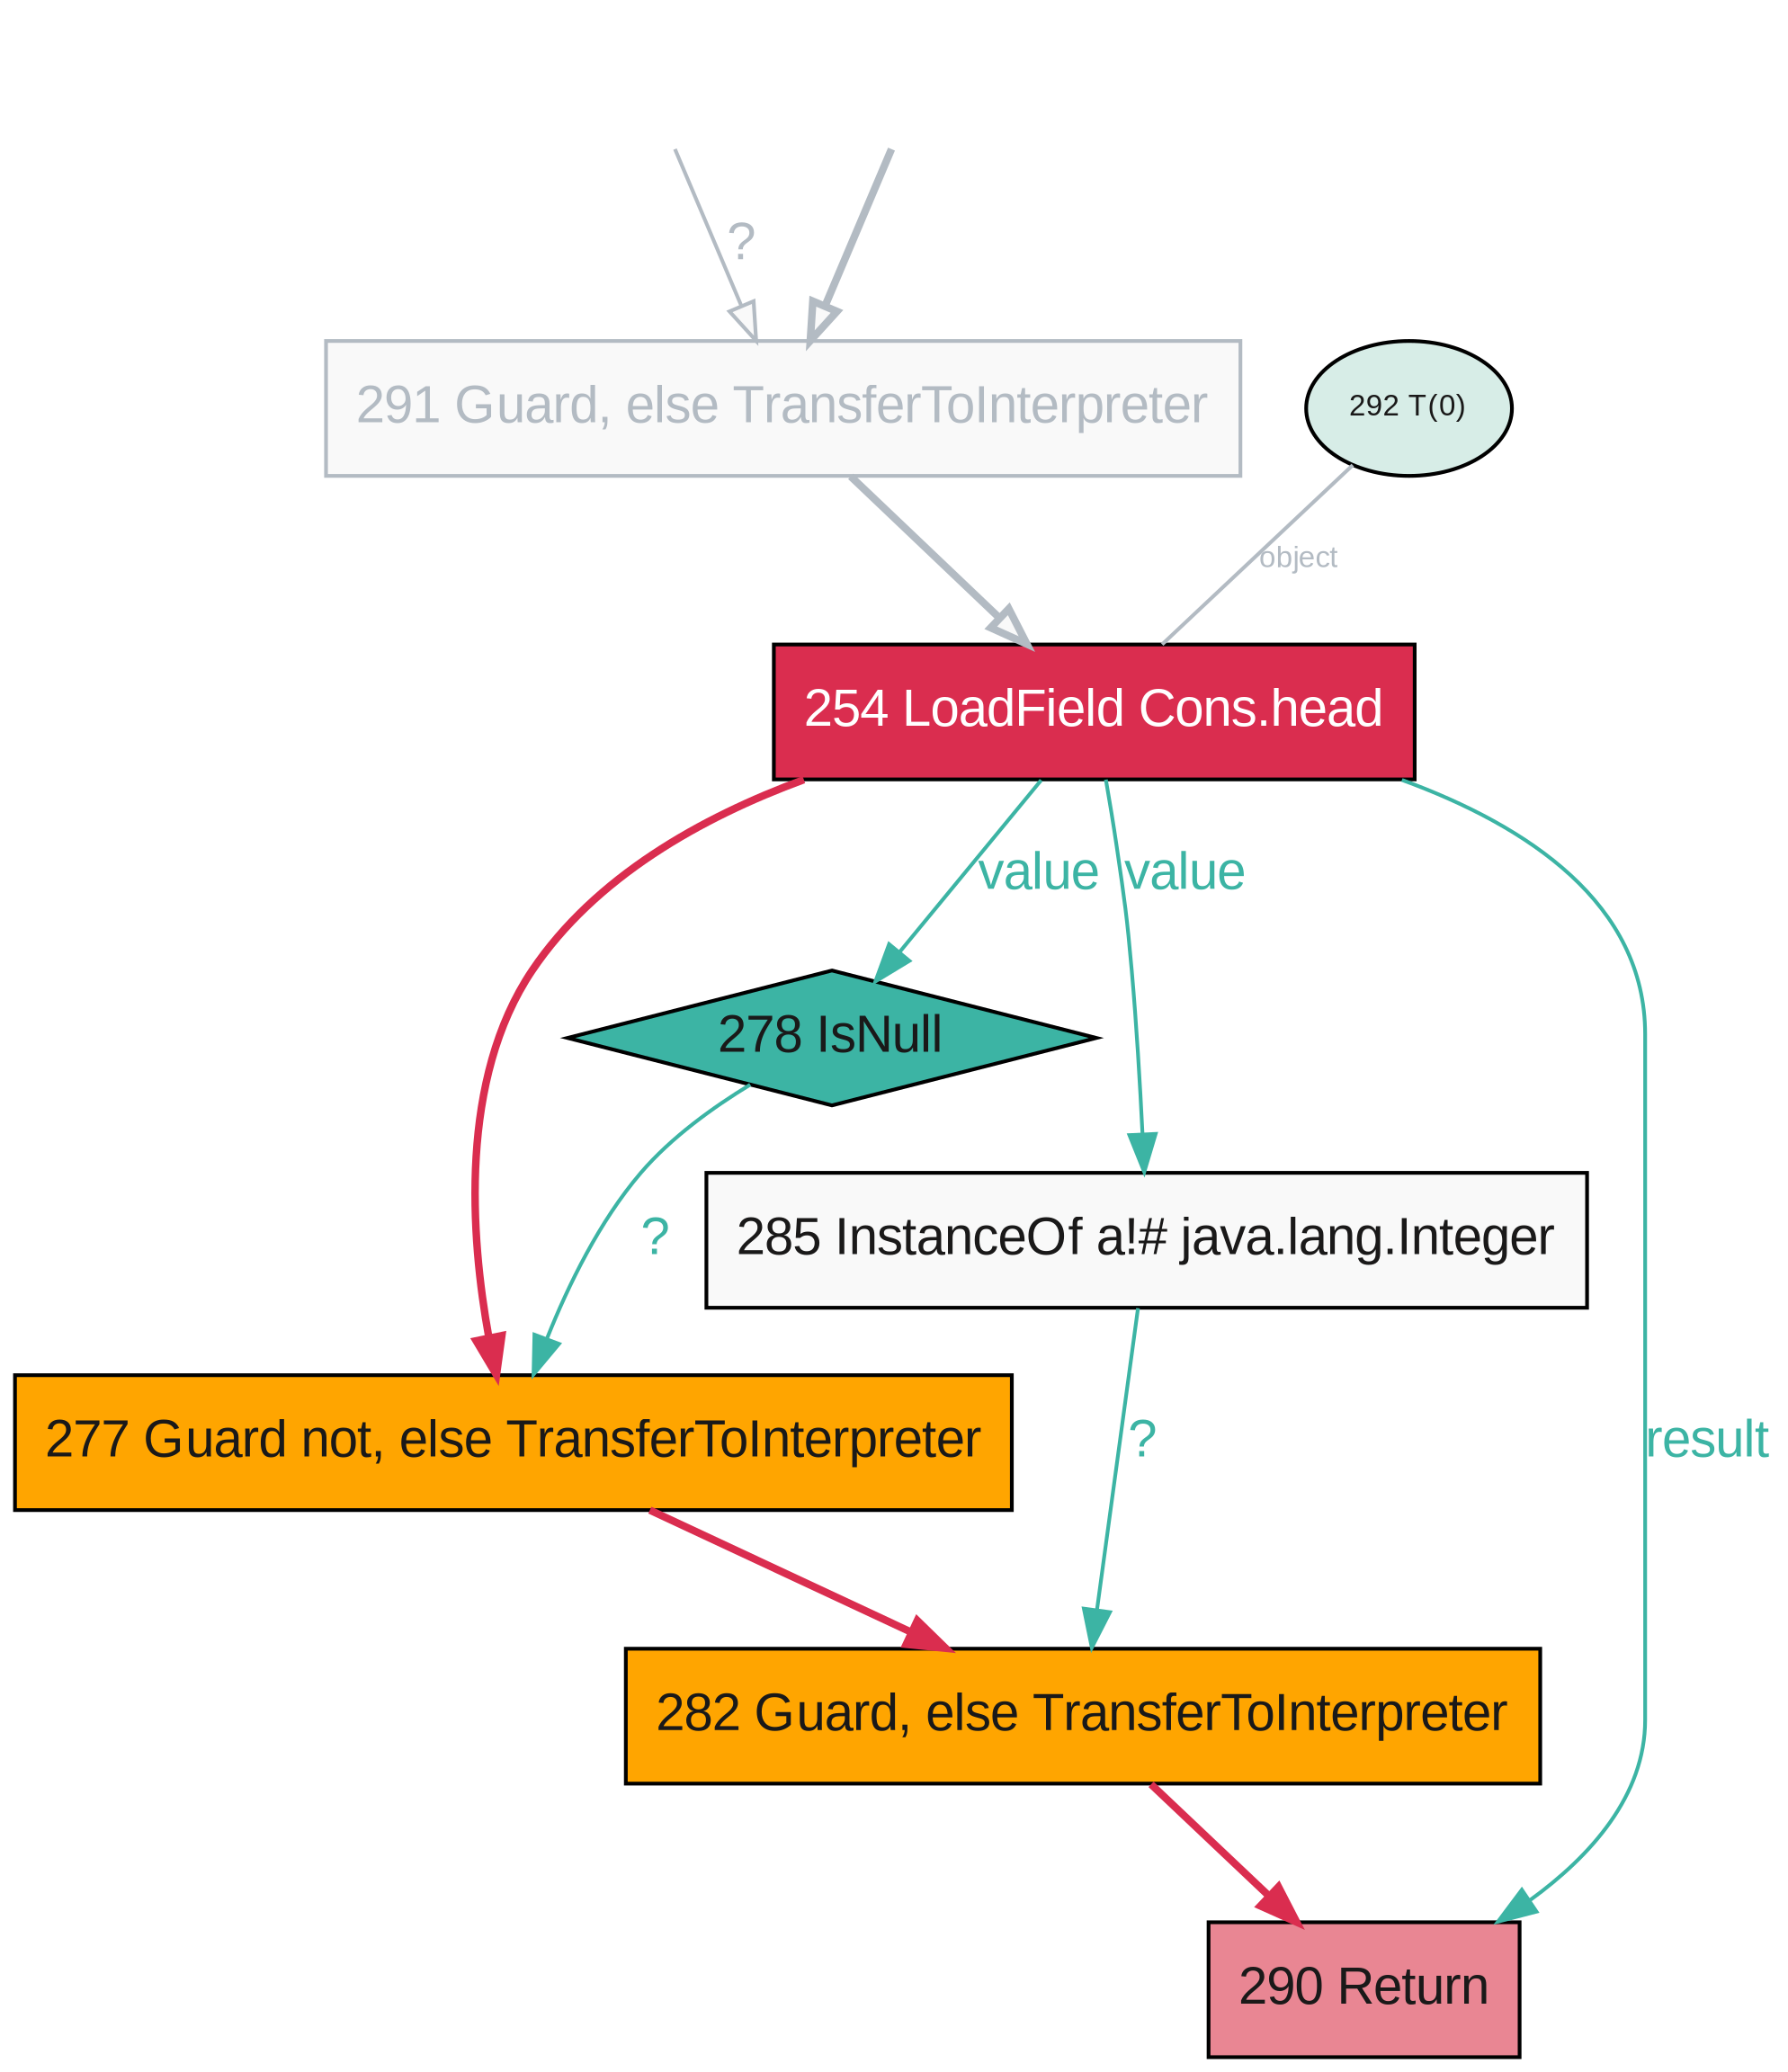
\includegraphics[width=\textwidth]{figures/dot/List.head.boxed.TruffleTier.png}
		\caption{Graal IR of \scalainline{Cons.head} focused on field access of \scalainline{head0}}
		\label{graalir:cons-head-boxed}
	\end{subfigure}
	\hfill
	\begin{subfigure}[b]{0.45\textwidth}
		\centering
		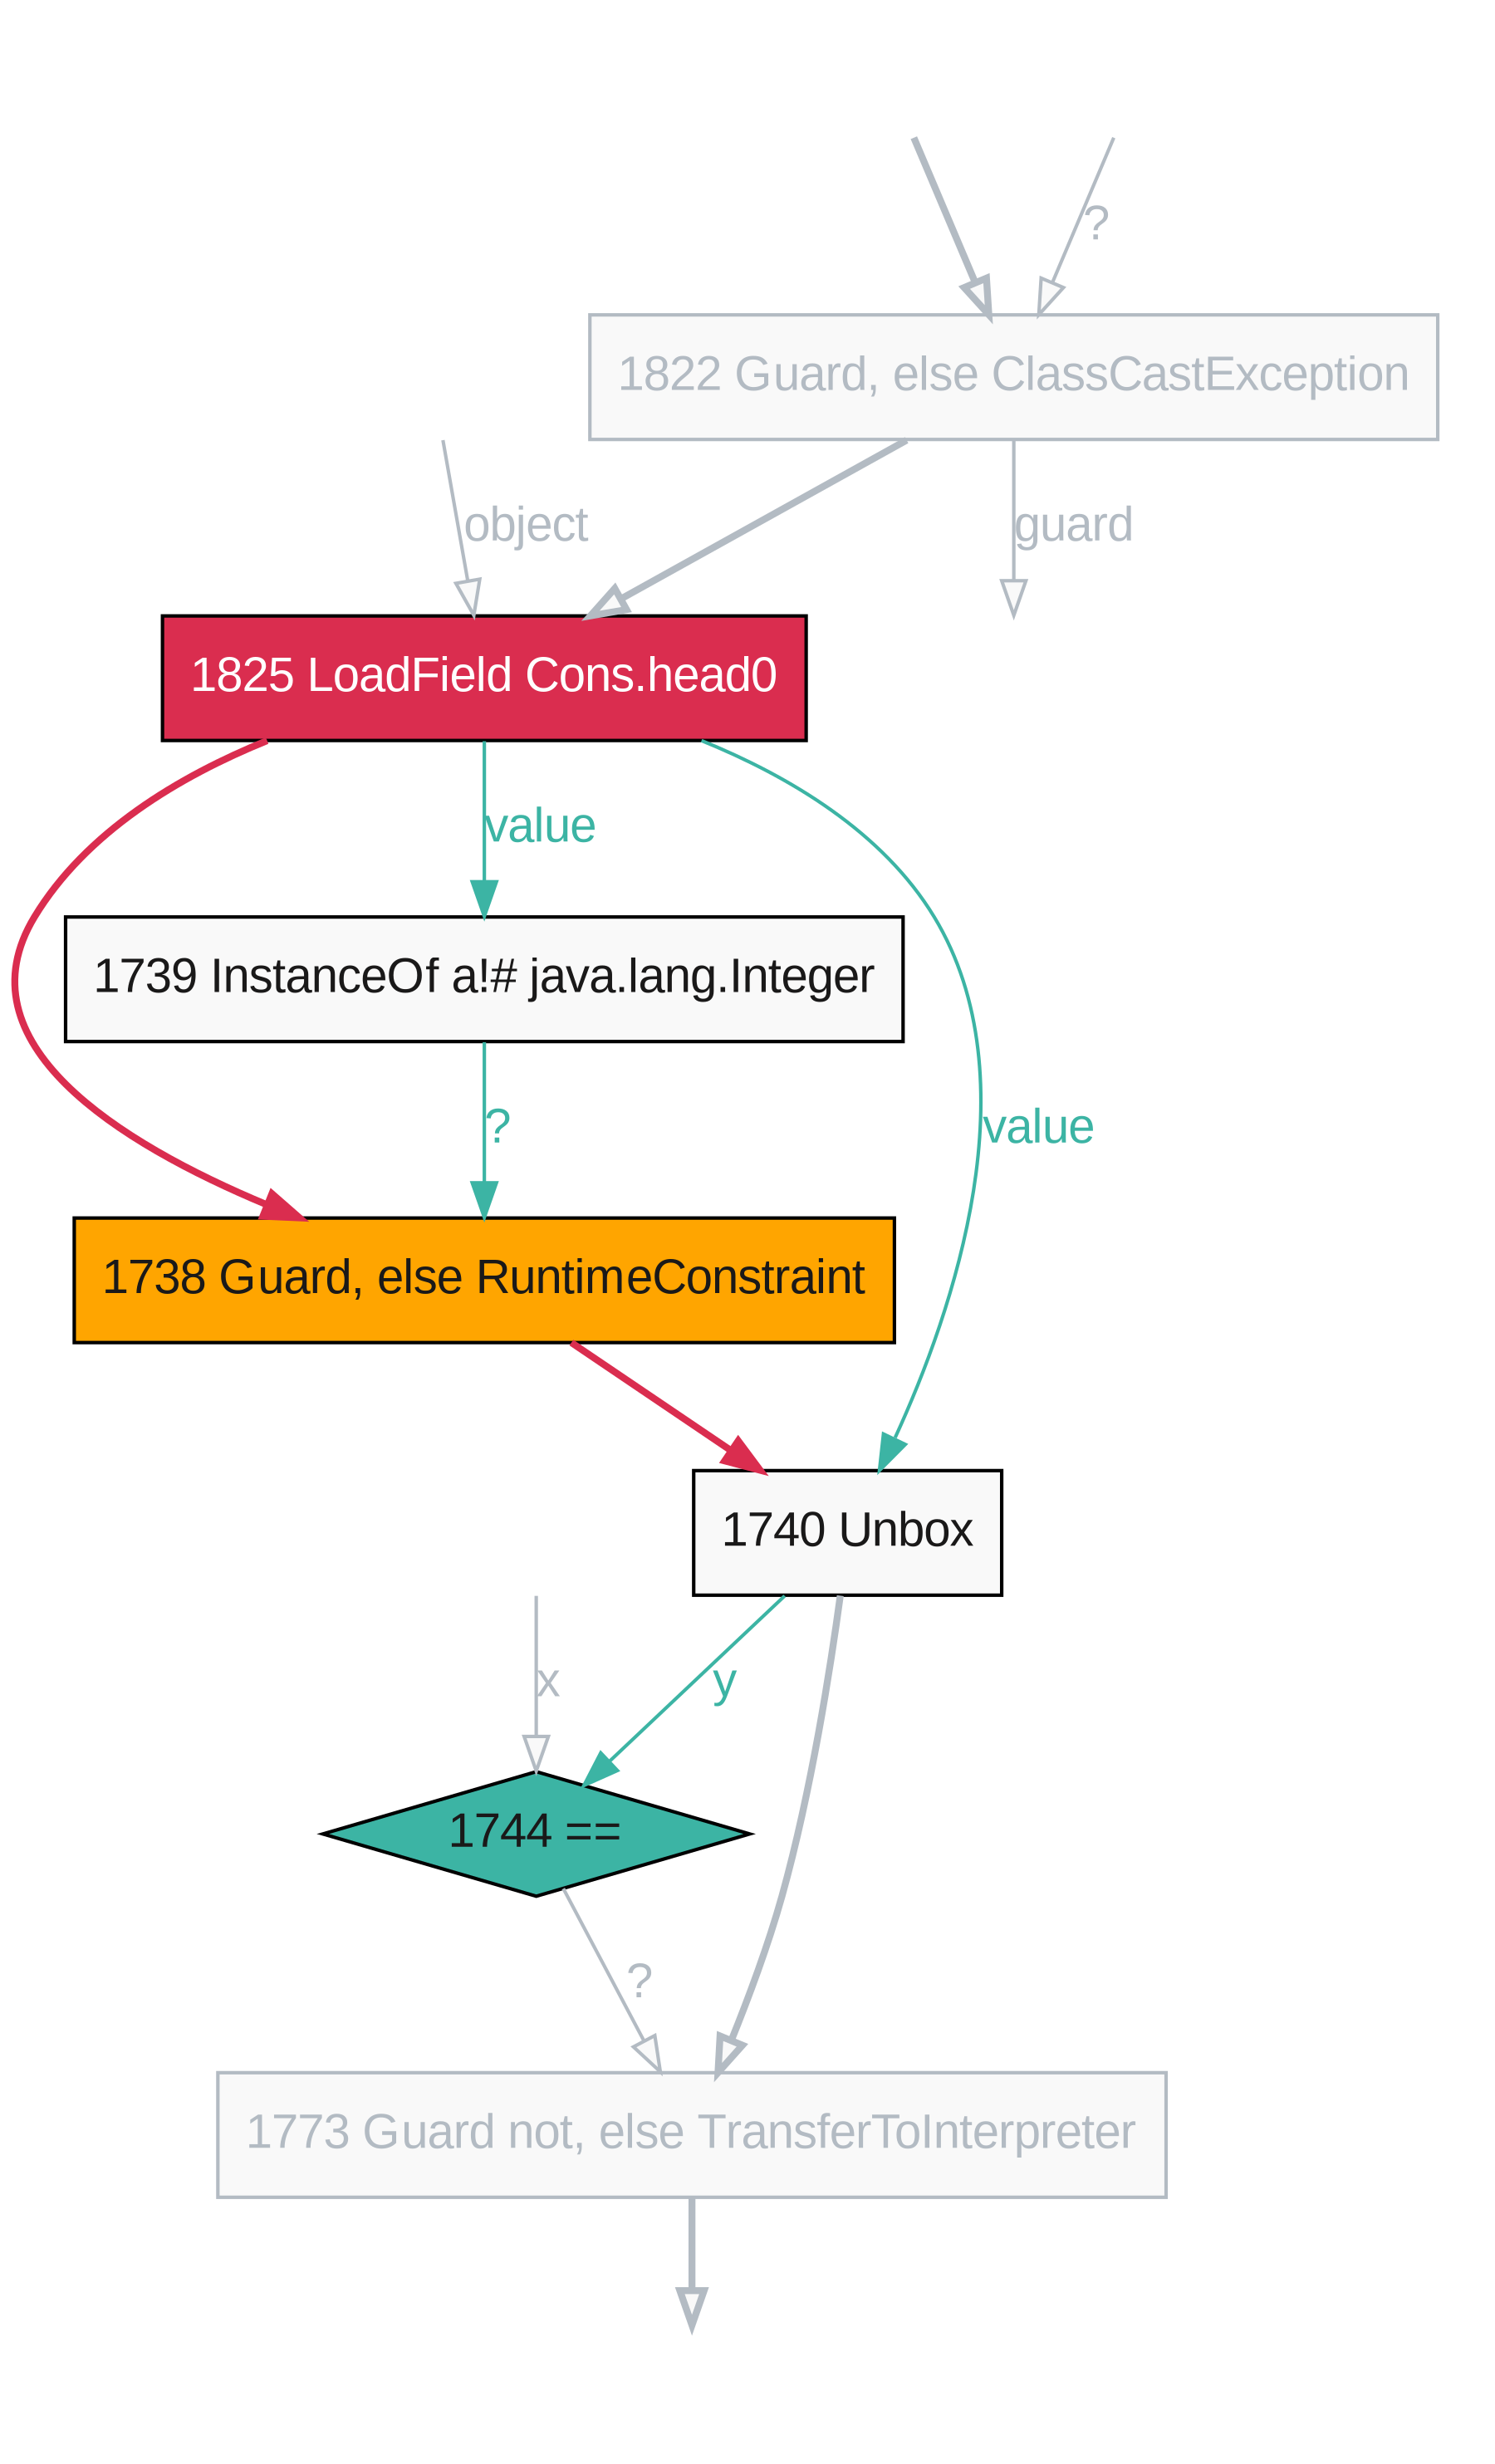
\includegraphics[width=\textwidth]{figures/dot/List.contains.boxed.TruffleTier.png}
		\caption{Graal IR of \scalainline{Cons.head} after being inlined into \scalainline{Cons.contains}}
		\label{graalir:cons-contains-head-focus-boxed}
	\end{subfigure}
	\hfill
\end{figure}

\subsection{Specializing Call Sites with \texttt{TypeApply} trees}

Generic methods in Scala can be polymorphic under class type parameters, method type parameters, or both. 
In the latter two cases, polymorphic methods contain additional reified type parameters. 
In addition to the polymorphic terms present in the method body discussed in the previous section, the type of method term parameters may be polymorphic. 
The following components of a generic method must specialized:

\begin{itemize}
	\item Polymorphic method parameters.
	\item Polymorphic terms inside the method body.
\end{itemize}


\subsubsection*{Method Parameters}

\subsubsection*{Typed Dispatch Chains}

Dispatch chains\cite{???}

\begin{figure}[!htb]
	\begin{minted}{scala}
	class TypeDispatchNode(parent: RootNode) extends TermNode {
		
		type TypeArguments: Array[Type]
		@CompilerDirectives.CompilationFinal
		var cache: Map[TypeArguments, DirectCallNode]
		
		override def execute(frame: VirtualFrame): Object = {
			val types: TypeArguments = resolveTypeParameters(frame)
			dispatch(frame, args);
		}
		
		def dispatch(frame: VirtualFrame, types: TypeArguments): Object = cache.get(types) match {
			case Some(callNode) => callNode.call(frame.getArguments)
			case None           => createAndDispatch(frame, types)
		}
		
		def createAndDispatch(frame: VirtualFrame, types: TypeArguments): Object = {
			CompilerDirectives.transferToInterpreterAndInvalidate()
			val specialization = parent.specialize(types)
			val callNode = DirectCallNode.create(specialization)
			cache = cache.updated(types, callNode)
			callNode.call(frame.getArguments)
		}
	}
	\end{minted}
\caption{Simplified implementation of generic dispatch node based on reified type arguments.}
\end{figure}

\begin{figure}[H]
	\centering
	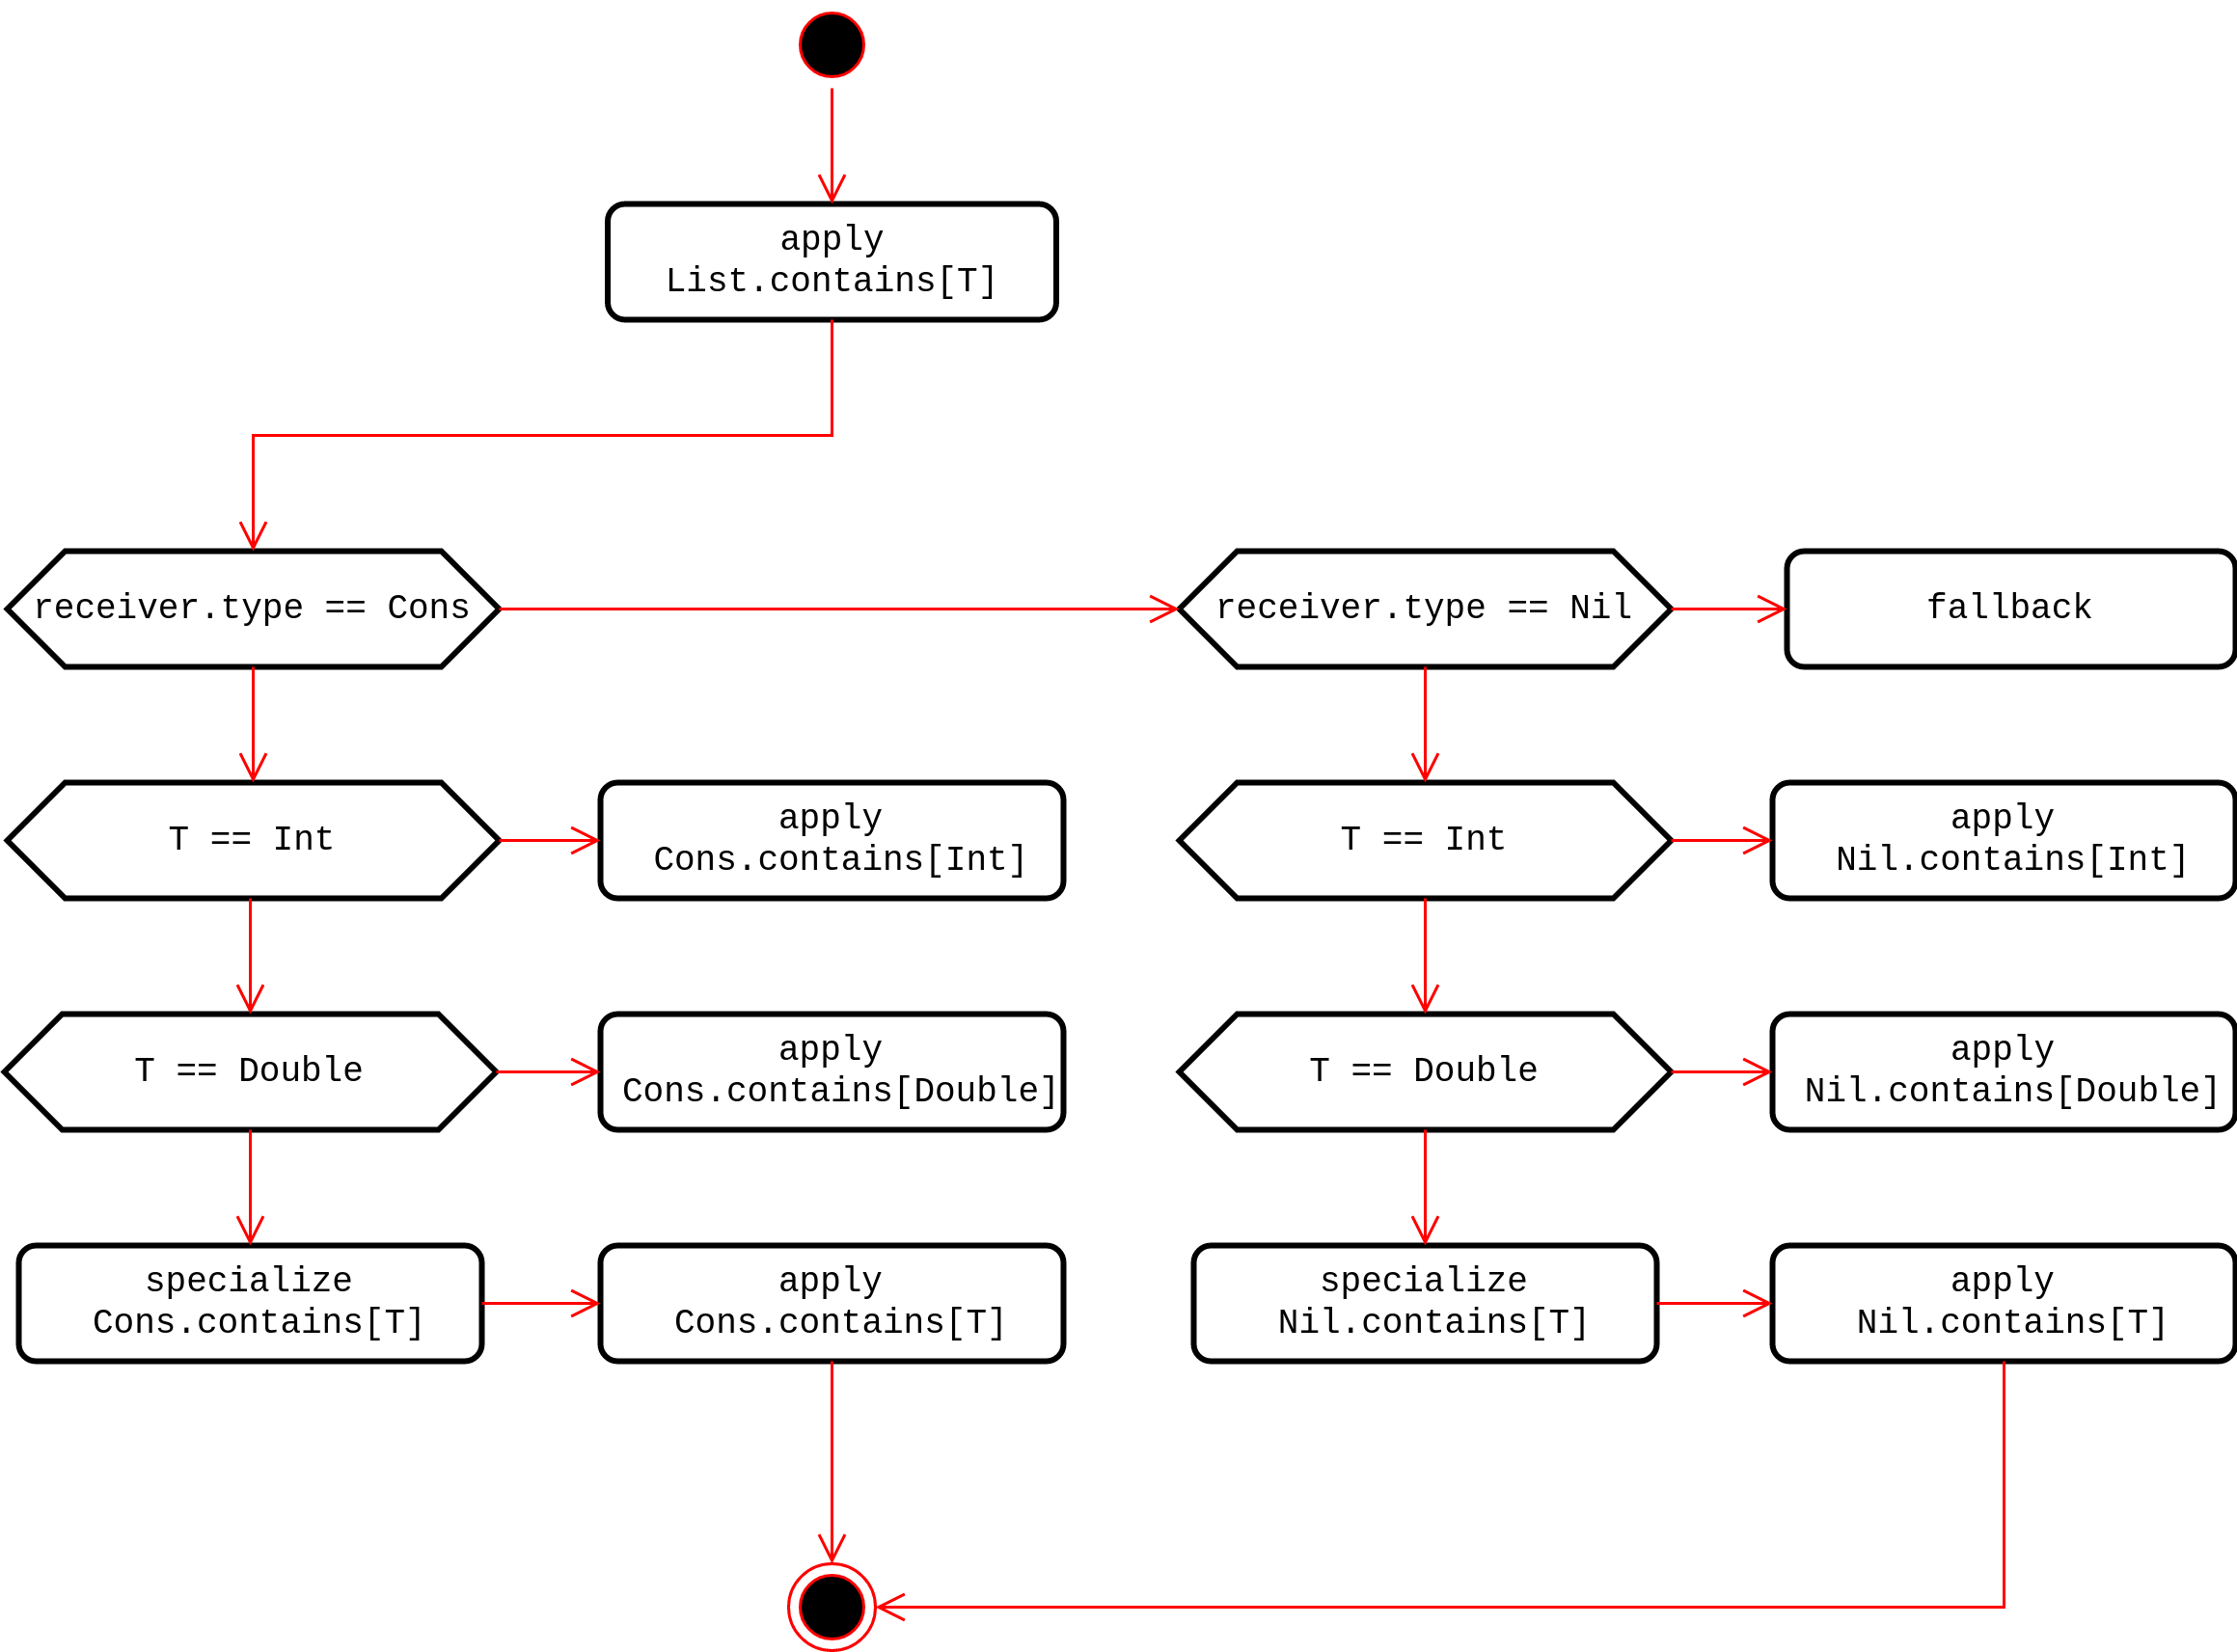
\includegraphics[width=0.75\textwidth]{figures/tastytruffle-type-dispatch-chain.png}
	\caption{The typed dispatch chain for a \scalainline{List.contains} call site }
\end{figure}

\subsubsection*{Code Duplication}

\subsubsection*{Partial Evaluation}

\subsection{Specializing Terms}

\begin{figure}[!htb]
	\centering
	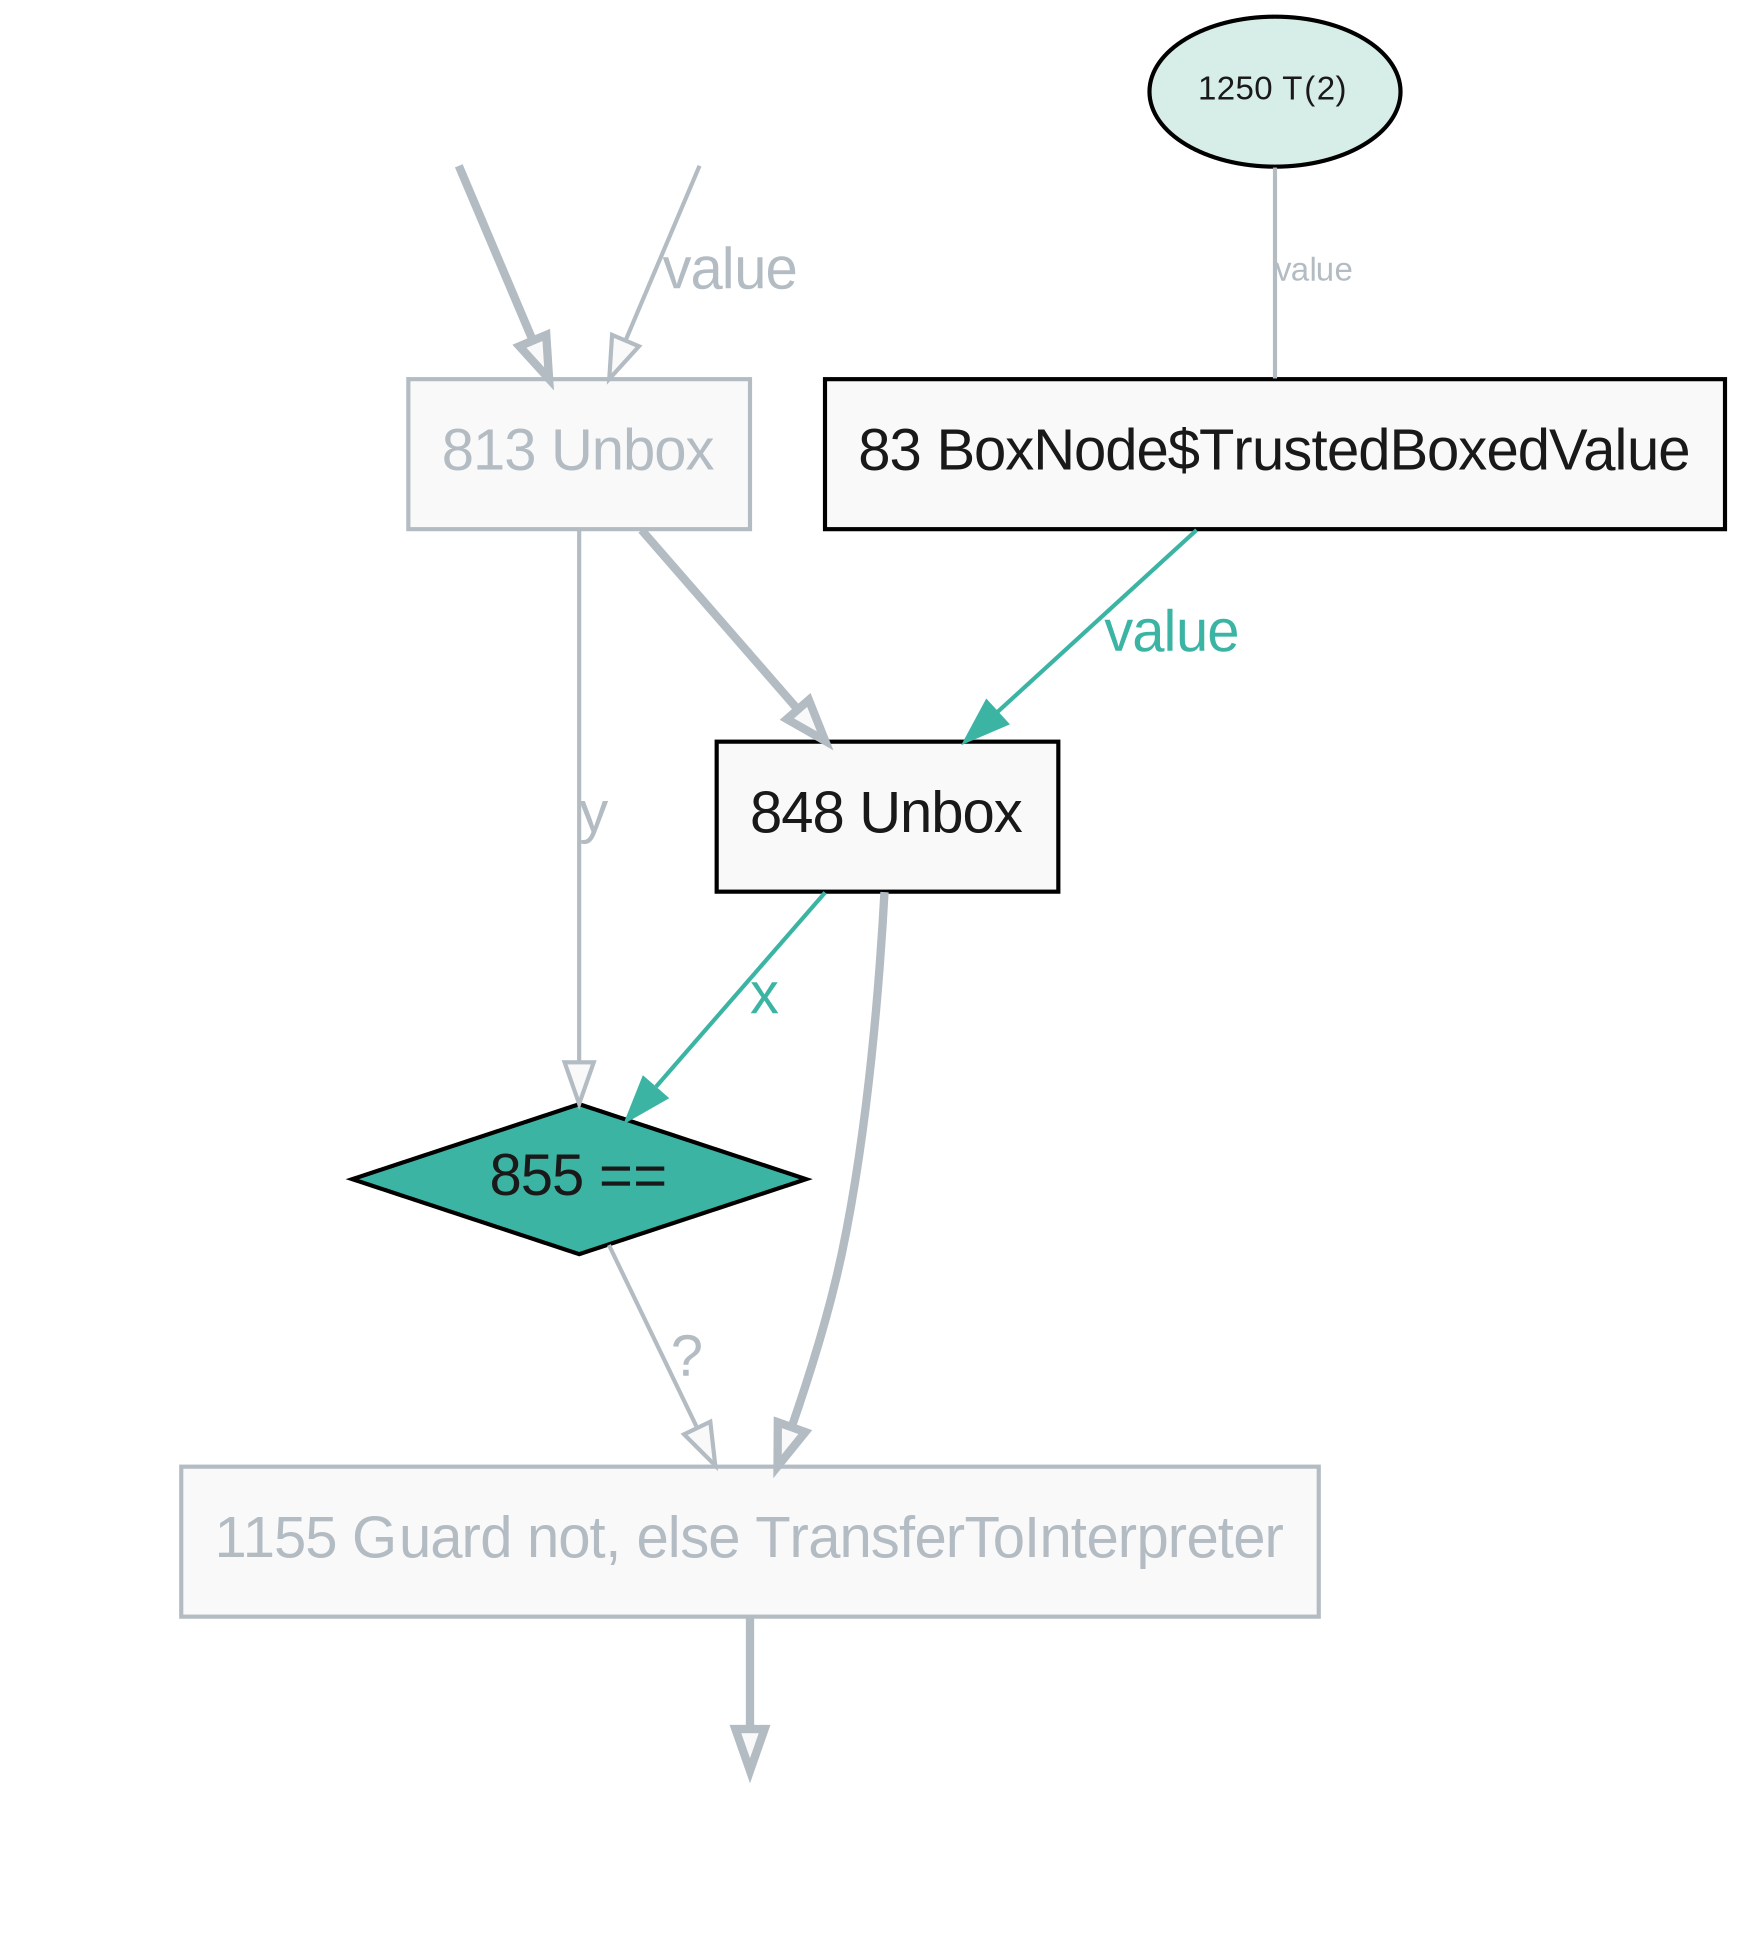
\includegraphics[width=0.4\textwidth]{figures/dot/List.contains.boxed-param-read.TruffleTier.png}
	\caption{Graal IR of \scalainline{List.head} after field read of \scalainline{head0} is specialized.}
	\label{graalir:cons-contains-param-read}
\end{figure}


\begin{figure}
	\centering
	\begin{subfigure}[b]{0.4\textwidth}
		\centering
		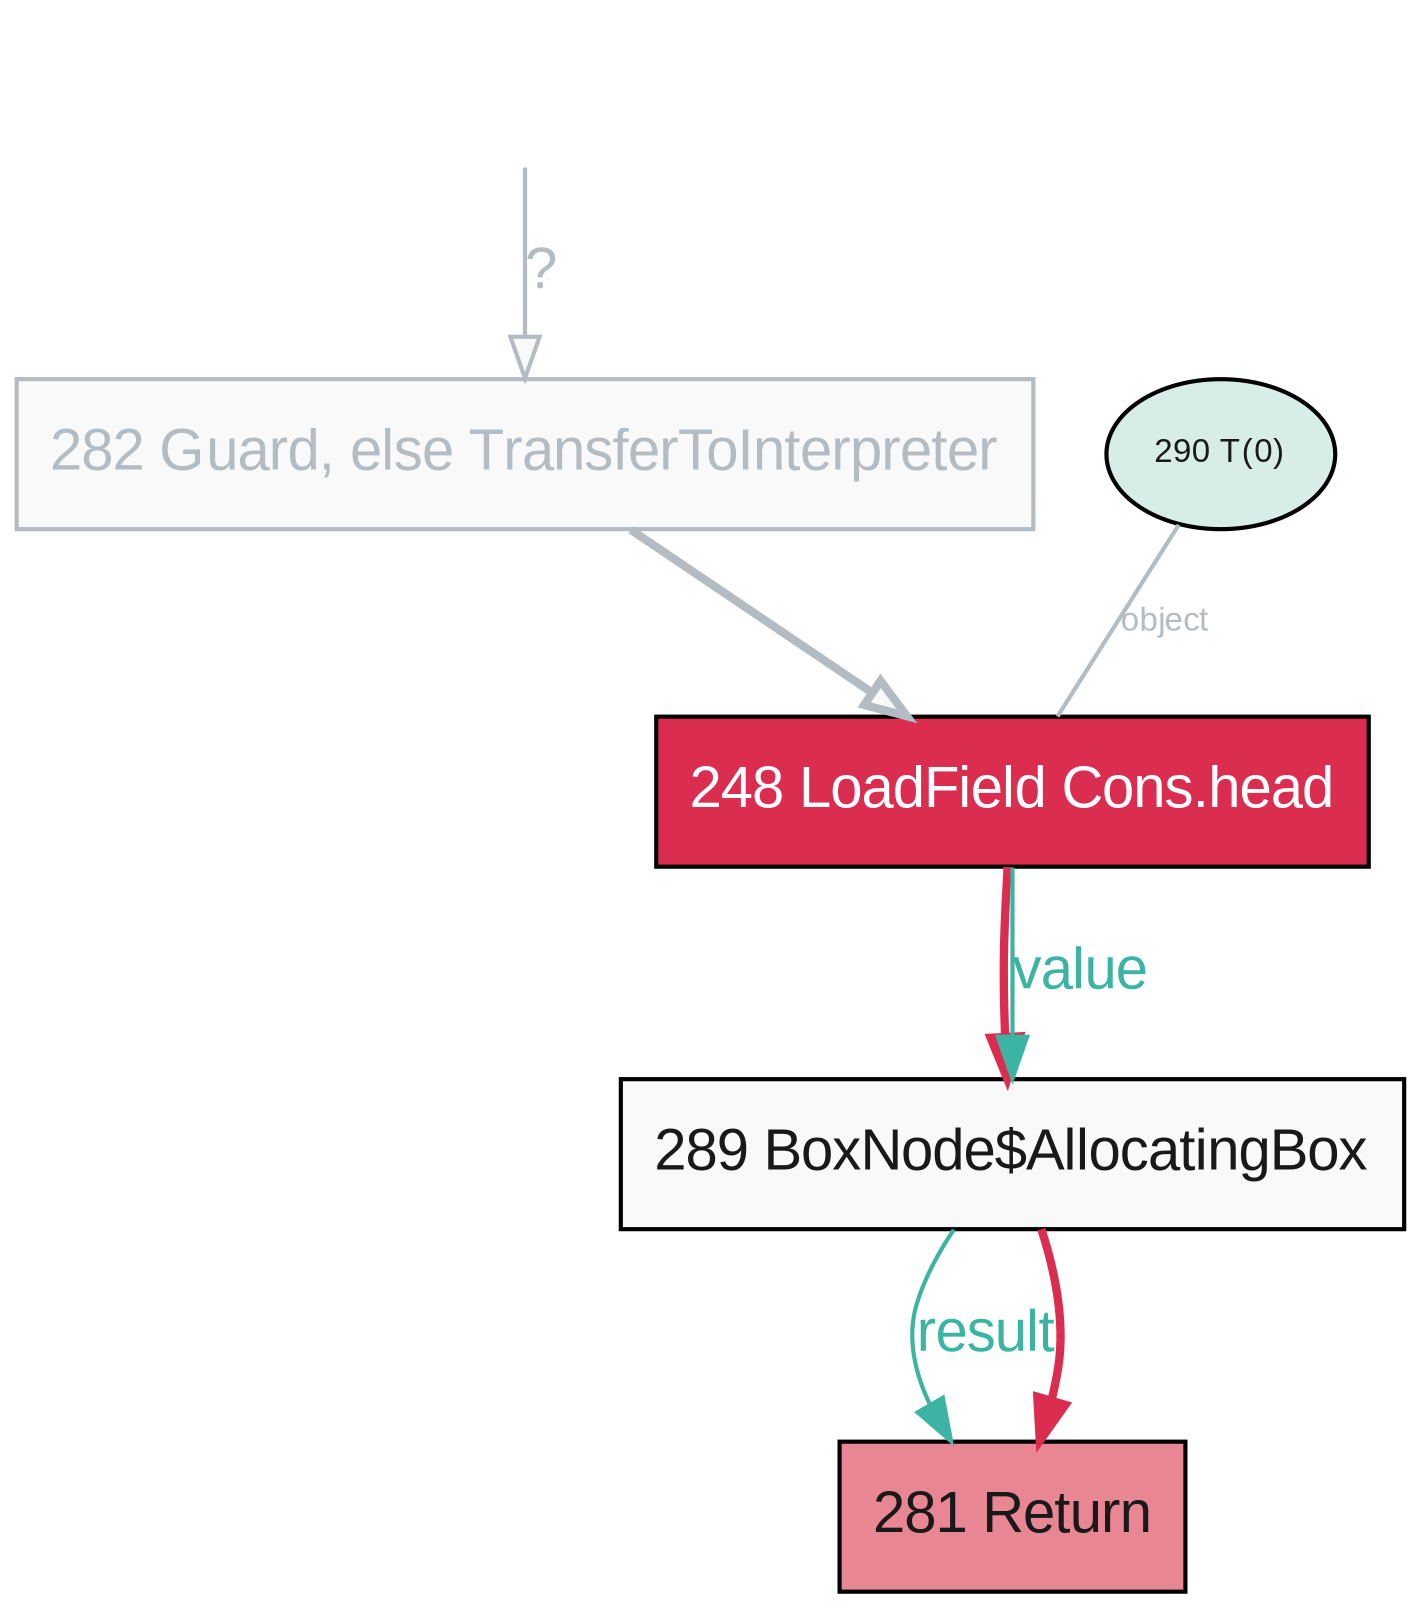
\includegraphics[width=\textwidth]{figures/dot/List.head.specialized.TruffleTier.png}
		\caption{Graal IR of \scalainline{List.head} after field read of \scalainline{head0} is specialized.}
		\label{graalir:cons-head-specialized}
	\end{subfigure}
	\hfill
	\begin{subfigure}[b]{0.4\textwidth}
		\centering
		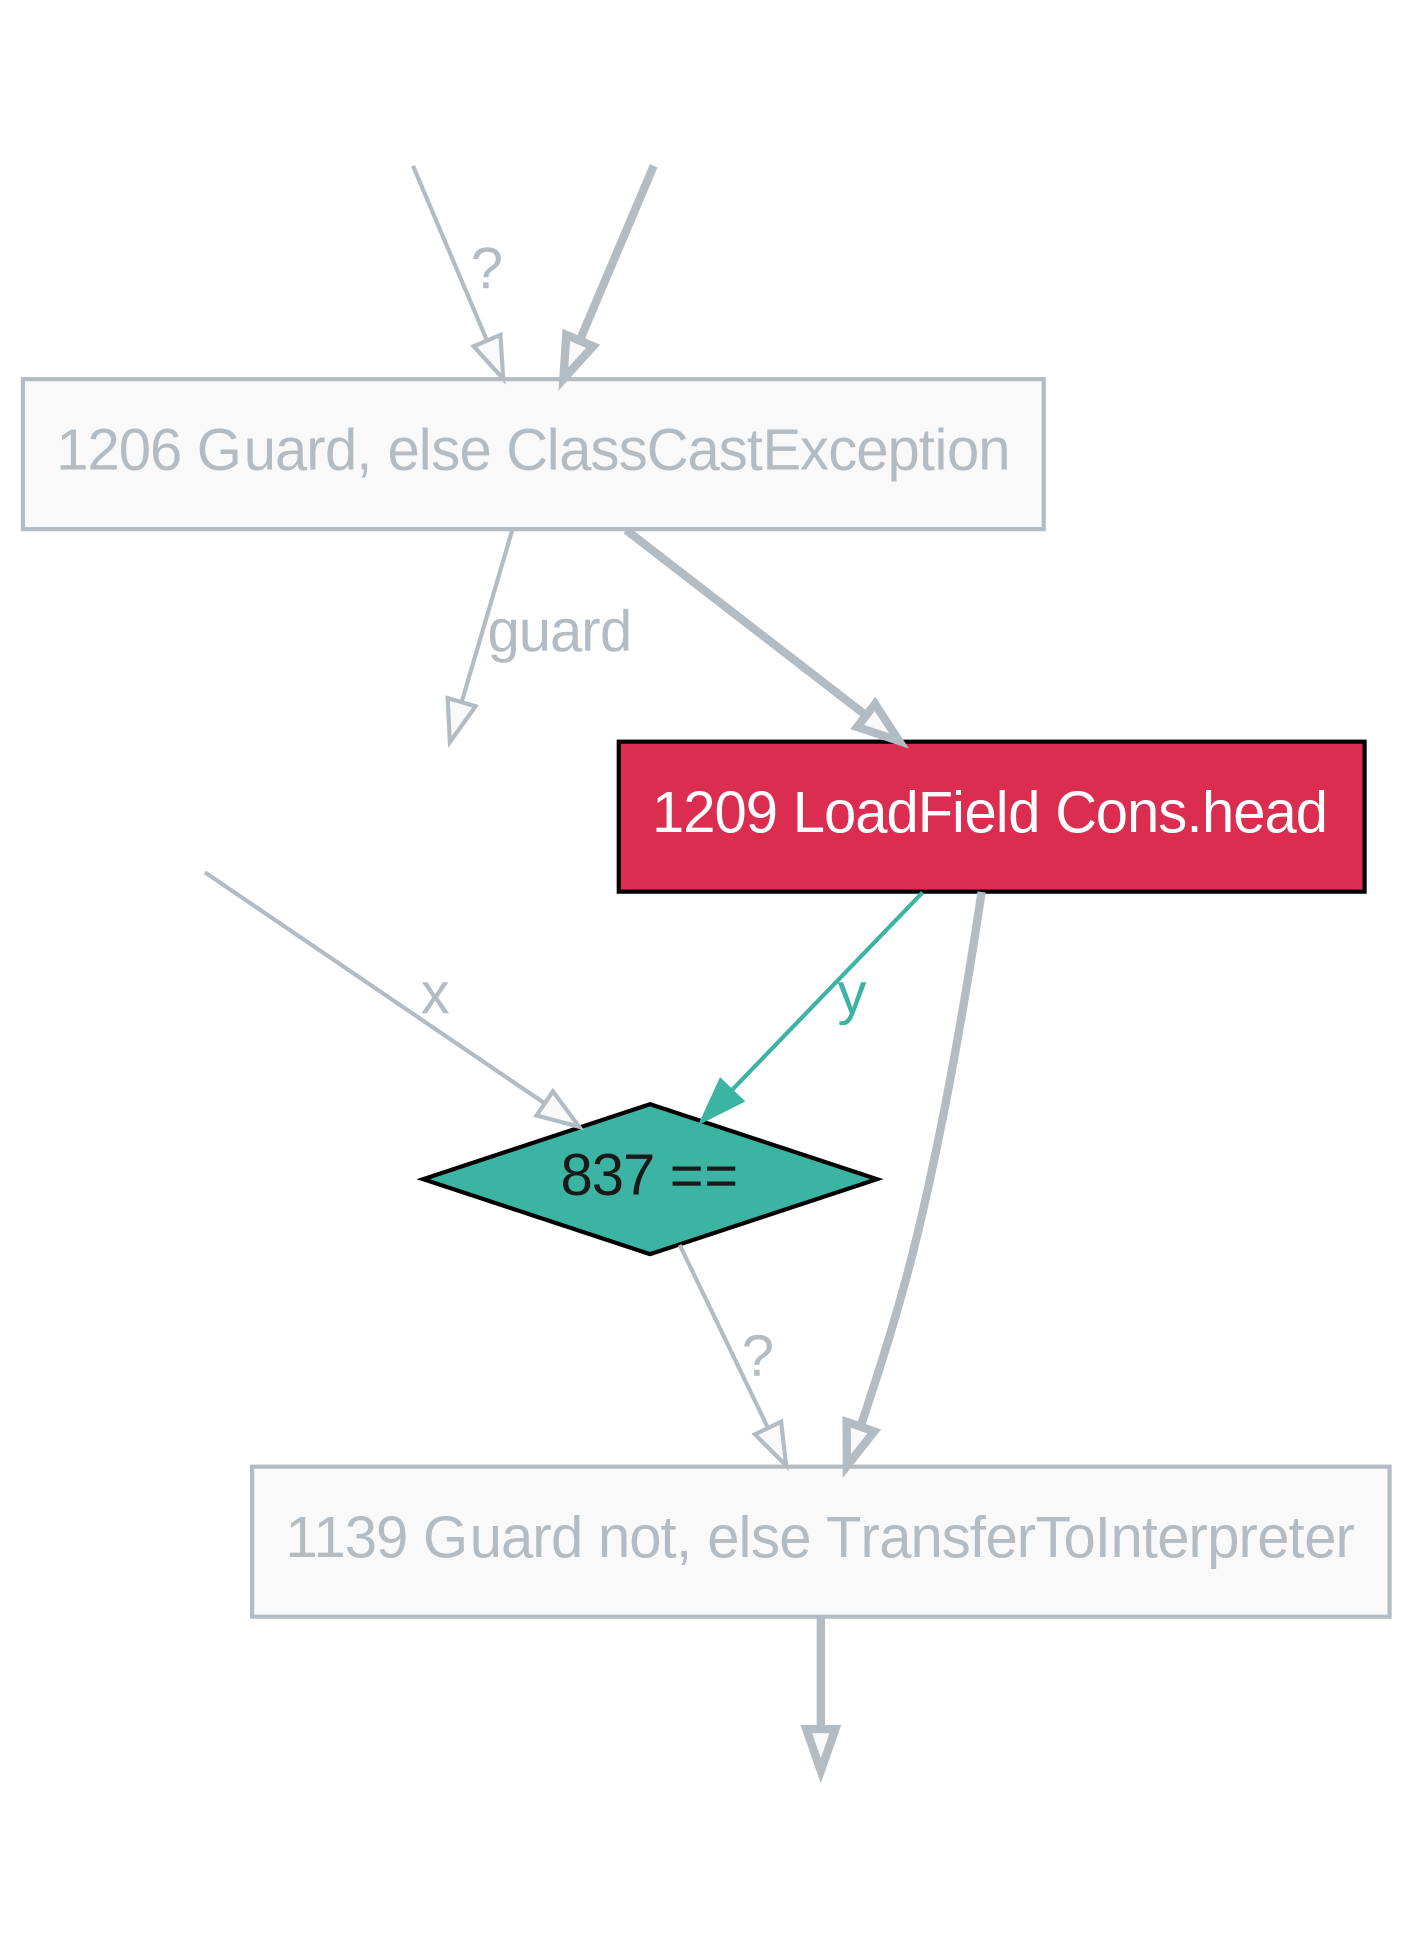
\includegraphics[width=\textwidth]{figures/dot/List.contains.specialized.TruffleTier.png}
		\caption{Graal IR of \scalainline{Cons.head} after being inlined into \scalainline{Cons.contains}}
		\label{graalir:cons-contains-head-focus-specialized}
	\end{subfigure}
	\hfill
\end{figure}


The basic polymorphic unit of code in Scala are terms whose types are derived directly from a type parameter \mintinline{scala}|T| or indirectly from a type constructor such as \mintinline{scala}|Array[T]|.
Polymorphic terms can be divided into the following categories:

\subsubsection*{Polymorphic local access}
\subsubsection*{Polymorphic field access}
\subsubsection*{Polymorphic method call}
\subsubsection*{Polymorphic instantiation}

